\documentclass{article}

\usepackage{fullpage}
\usepackage{amsmath,amsbsy,amsfonts,amssymb,amsthm}
\newtheorem{theorem}{Theorem}


\usepackage{graphicx}
\usepackage{dsfont}
\usepackage{algorithm}
\usepackage{algorithmic}
\usepackage{minted}
\usepackage{xcolor}
\usepackage{mdframed}

\newcommand{\field}[1]{\mathbb{#1}}
\newcommand{\set}[1]{\mathcal{#1}}
\newcommand{\fY}{\set{Y}}
\newcommand{\fX}{\set{X}}
\newcommand{\fF}{\set{F}}
\newcommand{\fH}{\set{H}}
\newcommand{\fD}{\set{D}}

\newcommand{\R}{\field{R}}
\newcommand{\Nat}{\field{N}}

\renewcommand{\Pr}{\field{P}}
\newcommand{\Ind}{\mathds{1}}
\newcommand{\E}{\field{E}}
\newcommand{\Var}{\mathrm{Var}}

\DeclareMathOperator*{\argmin}{arg\,min}
\DeclareMathOperator*{\argmax}{arg\,max}

\DeclareMathOperator{\sign}{sign}

\newcommand{\RiskD}{L_{\fD}}
\newcommand{\RiskS}{L_{S}}
\newcommand{\RiskSi}{L_{S_i}}
\newcommand{\RiskV}{L_{V}}
\newcommand{\RiskT}{L_{T}}

\newcommand{\blambda}{\boldsymbol{\lambda}}
\newcommand{\bnu}{\boldsymbol{\nu}}
\newcommand{\btheta}{\boldsymbol{\theta}}
\newcommand{\bx}{\boldsymbol{x}}
\newcommand{\bX}{\boldsymbol{X}}
\newcommand{\bw}{\boldsymbol{w}}
\newcommand{\bu}{\boldsymbol{u}}
\newcommand{\bv}{\boldsymbol{v}}
\newcommand{\by}{\boldsymbol{y}}
\newcommand{\bz}{\boldsymbol{z}}
\newcommand{\bV}{\boldsymbol{V}}
\newcommand{\bD}{\boldsymbol{D}}
\newcommand{\bphi}{\boldsymbol{\phi}}
\newcommand{\bPhi}{\boldsymbol{\Phi}}
\newcommand{\bxi}{\boldsymbol{\xi}}
\newcommand{\bbeta}{\boldsymbol{\beta}}
\newcommand{\balpha}{\boldsymbol{\alpha}}

\newcommand{\newdef}[1]{\textbf{#1}}

\newcommand{\norm}[1]{\left\lVert#1\right\rVert}

\DeclareMathOperator{\Conv}{conv}
\newcommand\braces[1]{\{#1\}}
\newcommand\brackets[1]{[#1]}
\newcommand\dotp[1]{\langle #1 \rangle}
\newcommand\Parens[1]{\mleft(#1\mright)}
\newcommand\Norm[1]{\mleft\|#1\mright\|}
\newcommand\Braces[1]{\mleft\{#1\mright\}}
\newcommand\Brackets[1]{\mleft[#1\mright]}
\newcommand\Ceil[1]{\mleft\lceil#1\mright\rceil}
\newcommand\Abs[1]{\mleft|#1\mright|}
\newcommand\Dotp[1]{\mleft\langle#1\mright\rangle}

\newcommand{\Proj}{\ensuremath{\operatorname{Proj}}}

\title{\bf Stony Brook University \\ CSE512 -- Machine Learning -- Spring 17 \\  
Homework 2, Due: March, 7, 2017, 11:59PM \\ Sudeshna Pal(110938222)}
\date{\vspace{-1cm}}

\begin{document}

\maketitle

\section*{Instructions}
\begin{itemize}
\item The homework is due on March 7, 2017. Anything that is received after the deadline will not be considered.
\item The write-up \textbf{must} be prepared in Latex, including the Matlab code and figures in the report.
\item We can use any Latex class you like, just report question number and your answer.
\item If the question requires you to implement a Matlab function, the answer should be your code. Make sure it is sufficiently well documented that the TAs can understand what is happening.
\item Each Question, regardless of how many sub-questions contains, is worth 10 points.
\end{itemize}

\section{Ridge Regression}
\subsection{Question 1}

In class, you learned about using $k$-folds cross validation as a way to estimate the true error of a learning algorithm and to tune parameters. The preferred solution is \emph{Leave-One-Out Cross Validation} (LOOCV), which provides an almost unbiased estimate of this true error, but it can take a really long time to compute. In this problem, you will derive an algorithm for efficiently computing the LOOCV error for a particular regression algorithm.

We will now introduce a simple extension of the Least Square algorithm.
Given a set of $m$ data points and associated labels $\{\bx_i, y_i | \bx_i \in \Re^d, y_i \in \Re \}_{i=1}^{m}$. \textbf{Ridge Regression} finds the weight vector $\bw$ and a bias term $b$ to optimize the following:
\begin{align}
 \label{eq:rr}
\min_{\bw, b} \ \lambda \|\bw\|^2 + \sum_{i=1}^{m} (\bw^\top\bx_i + b - y_i)^2~.
\end{align}
Note that with $\lambda=0$ Ridge Regression is exactly the Least Square formulation.

\begin{itemize}
\item Using the Matlab notation, let $\bar{\bw} = [\bw; b], \bar{X} = [X; \boldsymbol{1}^\top], \bar{I} = [I, \boldsymbol{0}; \boldsymbol{0}^\top, 0]$, $C = \bar{X} \bar{X}^\top + \lambda \bar{I}$, and $\boldsymbol{d} = \bar{X} \by$. Show that the solution of Ridge regression is: 
\begin{align}
\label{eq:sol_rr}
	\bar{\bw} = C^{-1} \boldsymbol{d}~.
\end{align}

\textbf{SOLUTION}
\begin{mdframed}[backgroundcolor=lightgray]
Ordinary least squares (ols) minimizes the sum of squared errors. However if there is a strong correlation between two parameters ols fails. So, ridge regression minimizes the squared error satisfying additional constraint that is $\sum_{i=1}^{P} w_i^2  \leq{c}$. \\
If number of parameters, $P = 2$, minimum squared error for ridge regression is:
\begin{flalign}
    min \sum_{i=1}^m(y_i - w_0 + w_1x_{1i} + w_2x_{2i})^2\\
    \text{constrained to}
    \sum_{i=1}^{2} w_i^2  \leq{c}
\end{flalign} 
By using Lagrange multiplier, the above equation becomes,
\begin{equation}
    min \sum_{i=1}^m(y_i - w_0 + w_1x_{1i} + w_2x_{2i})^2 + \lambda\big(\sum_{j=1}^2  w_i^2 - c\big)
\end{equation}
$\lambda$ and c are constants. So, we can write the above equation as
\begin{equation}
    min \sum_{i=1}^m(y_i - w_0 + w_1x_{1i} + w_2x_{2i})^2 + \lambda\big(\sum_{j=1}^2  w_i^2 \big)
\end{equation}
In matrix form,
\begin{equation}
    min (Y - \bar w^T \bar X) (Y - \bar w^T \bar X)^T + \lambda \bar w^T \bar w
\end{equation}
Conceptually, we understand that $\lambda \bar w^T \bar w$ would be the penalty paid highly correlated parameters. Now to find minimum we do partial derivative wrt. $\bar w$ and equating it to 0.\\
\begin{align}
    \frac{\partial}{\partial \bar w} &= 0\\
    -2\bar X Y + 2\bar X \bar X^T \bar w + 2 \lambda \bar w &= 0\\
    \bar w (\bar X \bar X^T + \lambda \bar I) &= \bar X Y \\
    \bar w &= (\bar X \bar X^T + \lambda \bar I)^{-1} \bar X Y
\end{align}
According to the question ${C = \bar X \bar X^T + \lambda \bar I}$ and $d = \bar X Y$, then the above equation becomes,
\begin{equation}
    \bar w = C^{-1}d
\end{equation}
\end{mdframed}


\item Now suppose we remove $\bx_i$ from the training data, let $C_{(i)}, \boldsymbol{d}_{(i)}, \bar{\bw}_{(i)}$ be the corresponding matrices for removing $\bx_i$. Express $C_{(i)}$ in terms of $C$ and $\bx_i$. Express $\boldsymbol{d}_{(i)}$ in terms of $\boldsymbol{d}$ and $\bx_i$. 

\textbf{SOLUTION}
\begin{mdframed}[backgroundcolor=lightgray]
After removing $x_i$ from training data, we know the corresponding rows and columns from matrices will be not present.
Hence, 
\begin{align*}
    d_{(i)} = d - x_i y_i.\\
    C_{(i)} = C - x_i x_i^T
\end{align*}
\end{mdframed}

\item Express $C_{(i)}^{-1}$ in terms of $C^{-1}$ and $\bx_i$.
\textsl{Hint:} use the Sherman-Morrison formula
\begin{align}
    (A + \bu\bv^\top)^{-1} = A^{-1} - \frac{A^{-1}\bu\bv^\top A^{-1}}{1 + \bv^\top A^{-1} \bu}~.
\end{align}

\textbf{SOLUTION}
\begin{mdframed}[backgroundcolor=lightgray]
\begin{align*}
    C_{(i)}^{-1} &= (C - x_i x_{(i)}^T)^{-1}\\
    C_{(i)}^{-1} &= (C + (-x_i) x_{(i)}^T)^{-1}\\
    &= \big( C^{-1} - \frac{C^{-1} (-x_{(i)}) x_{(i)}^T C^{-1} } {1 + x_{(i)}^T C^{-1} (-x_{(i)})} \big)
    &= 
\end{align*}
\end{mdframed}

\item Show that
\begin{align}
    \bar{\bw}_{(i)}  = \bar{\bw} + (C^{-1} \bar{\bx}_i)\frac{\bar{\bx}_i^\top\bar{\bw}-y_i}{ 1 - \bar{\bx}_i^\top C^{-1} \bar{\bx}_i}~.
\end{align}

\textbf{SOLUTION}
\begin{mdframed}[backgroundcolor=lightgray]
Substituting $\bar{w}$ with just $w$, $\bar{x}_i$ with just $x_i$ to make writing easy and the new solution after removing $x_i$ will be,
\[
C_i^{-1}d_i
\]

Substituting values of $C_i^{-1}$ and $d_i$ from previous section we get,
\[
w_i = (C^{-1} + \frac{C^{-1}x_ix_i^TC^{-1}}{1 - x_i^TC^{-1}x_i})(d - x_iy_i)
\]
\[
w_i = C^{-1}d + \frac{C^{-1}x_ix_i^TC^{-1}}{1 - x_i^TC^{-1}x_i}d - C^{-1}x_iy_i - \frac{C^{-1}x_ix_i^TC^{-1}}{1 - x_i^TC^{-1}x_i}x_iy_i
\]

Replacing $C^{-1}$ with $w$ and taking $C^{-1}x_i$ common, we get,

\[
w_i = w + C^{-1}x_i(\frac{x_i^TC^{-1}}{1 - x_i^TC^{-1}x_i}d - y_i - \frac{x_i^TC^{-1}}{1 - x_i^TC^{-1}x_i}x_iy_i)
\]
\[
w_i = w + C^{-1}x_i(\frac{x_i^TC^{-1}d - y_i + x_i^TC^{-1}x_iy_i - x_i^TC^{-1}x_iy_i}{1 - x_i^TC^{-1}x_i})
\]
\[ \pmb{
w_i = w + (C^{-1}x_i)(\frac{x_i^Tw - y_i}{1 - x_i^TC^{-1}x_i})} \tag {*} \label{*}
\]
\end{mdframed}

\item Show that the leave-one-out error for removing the $i^{th}$ training sample is
\begin{align}
\bar{\bw}_{(i)}^\top \bar{\bx}_i - y_i = \frac{\bar{\bw}^\top \bar{\bx}_i - y_i}{ 1 - \bar{\bx}_i^\top C^{-1} \bar{\bx}_i}~.
\end{align} 

\textbf{SOLUTION}
\begin{mdframed}[backgroundcolor=lightgray]
We know that the error is given by
\[
E = w_i^Tx_i - y_i
\]

Substituting the value of $w_i$ from previous answer,
\[
E = (w + (C^{-1}x_i)(\frac{x_i^Tw - y_i}{1 - x_i^TC^{-1}x_i}))^Tx_i - y_i
\]
\[
E = (w^T + ((C^{-1}x_i)(\frac{x_i^Tw - y_i}{1 - x_i^TC^{-1}x_i}))^Tx_i - y_i
\]
\[
E = (w^T + ((\frac{x_i^Tw - y_i}{1 - x_i^TC^{-1}x_i})^T(C^{-1}x_i)^T)x_i - y_i
\]
\[
E = (w^T + (\frac{(x_i^Tw - y_i)^T}{1 - x_i^TC^{-1}x_i})(x_i^T(C^{-1})^T)x_i - y_i
\]
\[
E = (w^T + (\frac{(x_i^Tw)^T - y_i^T}{1 - x_i^TC^{-1}x_i})(x_i^T(C^{-1})^T)x_i - y_i
\]
\[
E = (w^T + (\frac{w^Tx_i - y_i^T}{1 - x_i^TC^{-1}x_i})(x_i^T(C^{-1})^T)x_i - y_i
\]
\[
E = \frac{(w^T(1 - x_i^TC^{-1}x_i) + (w^Tx_i - y_i^T)(x_i^T(C^{-1})^T)x_i - y_i(1 - x_i^TC^{-1}x_i)}{1 - x_i^TC^{-1}x_i}
\]

We know that $C$ is symmetric and hence we can replace $C^T$ with $C$ and also, we know that $(C^{-1})^T = (C^T)^{-1} = C^{-1}$. Therefore,
\[
E = \frac{(w^T(1 - x_i^TC^{-1}x_i) + (w^Tx_i - y_i^T)(x_i^TC^{-1})x_i - y_i(1 - x_i^TC^{-1}x_i)}{1 - x_i^TC^{-1}x_i}
\]

\[
E = \frac{w^Tx_i - y_i}{1 - x_i^TC^{-1}x_i} \label{*} \tag{*}
\]

Substituting the above value in error equation, we get
\[ \pmb{
w_i^T - y_i = \frac{w^Tx_i - y_i}{1 - x_i^TC^{-1}x_i}} \label{*} \tag{*}
\]
\end{mdframed}

\item The LOOCV is defined as: 
$\sum_{i=1}^{m}(\bar{\bw}_{(i)}^\top\bar{\bx}_i - y_i)^2$. What is the algorithmic complexity of computing LOOCV error using the formula given in the previous point? How is it compared with the usual way of computing LOOCV?
Note that the complexity of inverting a $k\times k$ matrix is $O(k^3)$.

\begin{mdframed}[backgroundcolor=lightgray]
If we use the normal approach , then at every step we will end up spending minimum of $O(n^3)$ time for computing inverse of matrix. Therefore the total complexity will be $O(n^3)$. However, in the ridge regression all we need to do is to do matrix multiplications and addition. Therefore the time complexity of the new approach will be $O(n^2)$.
\end{mdframed}
\end{itemize}


\subsection{Question 2}
Implement the Ridge Regression algorithm that finds the solution of \eqref{eq:rr} through \eqref{eq:sol_rr}.
The prototype of the function must be 
\begin{verbatim}
[w,w_0] = train_rr(X, y, lambda)
\end{verbatim}
where $X \in \R^{m \times d}$ is the matrix of $m$ input vectors in $d$ dimension, i.e. each input $\bx_i$ is a row of $X$, $y$ is a column vector of $m$ columns containing the labels associated to the training samples. lambda is the value of $\lambda$ in \eqref{eq:rr}. You can assume $\lambda>0$.

\textbf{SOLUTION}
\begin{minted}[frame=single,framesep=10pt]{matlab}
function [w, w_0] = train_rr (X, Y, lambda)

    
    IdentityMatrix = eye(size(X,2));
    C = X' * X + (lambda * IdentityMatrix);
    d = X' * Y;
    
    w = pinv(C) * d;

    w_0 = w(1);
    w = w(2:size(w, 1));
end
\end{minted}


\section{Perceptron}

Given a sequence of $m$ samples $(\bx_i, y_i)$, where $\bx_i \in \R^d$ and the labels $y_i \in \{-1, 1\}$, the Perceptron algorithm
runs as follows:

\begin{algorithm}
\begin{algorithmic}
\STATE{Initialize: $\bw = 0$}
\FOR{$i = 1, \cdots, T$}
\IF{$y_i \langle \bw, \bx_i\rangle < 0$}
\STATE{$\bw \leftarrow \bw + y_i \bx_i$}
\ENDIF
\ENDFOR
\end{algorithmic}
\label{algo:perc}
\caption{Perceptron pseudocode}
\end{algorithm}

For simplicity, we have put the bias $b$ into $\bw$, that is $\bw \leftarrow [\bw; b]$ and $\bx_i \leftarrow [\bx_i ; 1]$. So it is no necessary
to consider the bias term in next two questions.
Assume $\|\bx_i\|\leq R$ for all $i$. We have shown that if there exists some $w^*$ such that $\|w^*\|=1$ and for all $i$
$y_i\langle w^*,\bx_i\rangle\geq\gamma$,
then the number of mistakes is upper bounded by
\begin{equation}
\label{eq:perc_bound}
\frac{R^2}{\gamma^2}~.
\end{equation}

\subsection{Question 3}
Consider the generalized Perceptron updates $\bw \leftarrow \bw + \eta y_i \bx_i$ with \emph{learning rate} $\eta > 0$. The Perceptron algorithm is the special case $\eta = 1$. Prove a bound on the number of mistakes similar to \eqref{eq:perc_bound}. How does $\eta$ affect this bound?

$\newline$
\textbf{SOLUTION}
\begin{mdframed}[backgroundcolor=lightgray]
Update rule given:
\[w_{(i+1)} = w_i + \eta x_iy_i\]

Therefore
\[||w_{(i+1)}||^2_2 = ||w_i||^2 + 2\eta y_i <w_i, x_i> + ||x_i||^2_2\]

\[ \leq ||w_i||^2 + \eta^2 R^2\]

Assuming M mistakes are made, we can write

\[||w_{(T+1)}||^2_2 \leq M \eta^2 R^2\]

Consider $w^*$ to achieve maximum in the definition of B

\[ <w^*, w_T+1> \leq ||w^*||_2 ||W_{T+1}||_2 \leq \eta R \sqrt{M}\]

Also consider 

\[ <w^*, w_T+1> = (w^*, + \sum_{t:mistakes on x_t} \eta y_t <w^*, x_t>) \geq \eta \gamma M \]

\[ <w^*, w_T+1> \geq  \eta \gamma M \]

putting it together

\[ \eta \gamma M \leq \eta R \sqrt{M} \]

Canceling $\eta$ and simplification gives us

\[ M \leq \frac{R^2}{\gamma^2}\]

Thus the $\eta$ factor does not affect the bound.
\end{mdframed}

\subsection{Question 4}
Now let's drop the assumption that samples are linear separable.
Let $\bu$ be any vector with $\|\bu\| = 1$ and let $\gamma > 0$. Define $\ell_i(\bu) = \max(0, \gamma - y_i\langle \bu, \bx_i\rangle)$ and and $L_q(\bu)=\sum_{i=1}^m \ell_i(\bu)^q$ for $1\leq q\leq 2$.
\begin{itemize}
\item Building on the previous proof, use the fact that you can express the updates \emph{on all rounds} as $\bw\leftarrow \bw + \tau_i y_i \bx_i$ for $\tau_i \in \{0,1\}$, and show that the number of mistakes $M$ of the Perceptron algorithm satisfies the \emph{implicit} (i.e. $M$ appears on both sides) inequality
\begin{equation}
\label{eq:implicit_M}
\gamma M\leq M^{1-\frac{1}{q}} L^\frac{1}{q}_q(\bu) + R\sqrt{M}, \ \forall 1 \leq q\leq 2
\end{equation}
\textsl{Hint:} Start from the proof seen in class, and use the H\"{o}lder's inequality:
\[
\sum_{i=1}^m a_i b_i \leq \left(\sum_{i=1}^m |a_i|^q\right)^\frac{1}{q} \left(\sum_{i=1}^m |b_i|^p\right)^\frac{1}{p}, \ \forall p,q\in[1,+\infty] \text{ such that } \frac{1}{p}+\frac{1}{q}=1~.
\]
Note that the Cauchy-Schwarz inequality is a special case of H\"{o}lder's inequality with $p=q=2$.\\

\textbf{SOLUTION}
\begin{mdframed}[backgroundcolor=lightgray]
\begin{align*}
   \|w_i+1\|^2  & = \|w_i\|^2 + 2 y_i \langle w_i, x_i \rangle + \|x\|^2 \\
   & \leq \|w_i\|^2 + R^2  , \text{ since } \ 2 y_i \langle w_i, x_i \rangle \leq 0 \text{ and  } \|x\|^2 \leq R^2 \\ 
   \ \langle w^*, w_T+1 \rangle & \leq R\sqrt{M} \\
   \\
   \ \langle w^*, w_T+1 \rangle & = \langle w^*,\sum _t  y_t x_t \rangle \\
   \ & = \sum _t y_t \langle w^*, x_t \rangle \\
   \ & = \sum_{i=1}^M \gamma - \ell_i(\bu) \\
   \ & = M \gamma - \sum_{i=1}^M \ell_i(\bu) \\
   \ & = M \gamma - \sum_{i=1}^M \ell_i(\bu) * 1 \\
   \ & \geq M \gamma - \left(\sum_{i=1}^m \ell_i(\bu)^q\right)^\frac{1}{q} \left(\sum_{i=1}^m |1|^p\right)^\frac{1}{p}, \ \forall p,q\in[1,+\infty] \text{ such that } \frac{1}{p}+\frac{1}{q}=1~. \\
   \ & \geq M \gamma - \left(\sum_{i=1}^m \ell_i(\bu)^q\right)^\frac{1}{q} \left(\sum_{i=1}^m |1|^{1-\frac{1}{q}}\right)^{1-\frac{1}{q}} , \ \forall 1 \leq q\leq 2 \\
   \ & \geq M \gamma - L^\frac{1}{q}_q(\bu) M^{1-\frac{1}{q}} , \ \forall 1 \leq q\leq 2 \\
   R\sqrt{M} & \geq M \gamma - L^\frac{1}{q}_q(\bu) M^{1-\frac{1}{q}} , \ \forall 1 \leq q\leq 2 \\ 
   M \gamma & \leq R\sqrt{M} + L^\frac{1}{q}_q(\bu) M^{1-\frac{1}{q}} , \ \forall 1 \leq q\leq 2 \\ 
\end{align*}  
\end{mdframed}

\item Setting $q=2$ in above, find an \emph{explicit} upper bound on $M$, that is $M$ must be only on the left hand side of the inequality.\\
\textbf{SOLUTION}
\begin{mdframed}[backgroundcolor=lightgray]
 \begin{align*}
M \gamma & \leq R\sqrt{M} + L^\frac{1}{q}_q(\bu) M^{1-\frac{1}{q}} , \ \forall 1 \leq q\leq 2 \\ 
M \gamma & \leq R\sqrt{M} + \sqrt{L_2(\bu)} \sqrt{M} , \text{ when q = 2 } \\ 
M \gamma & \leq \sqrt{M} (R + \sqrt{L_2(\bu)}) \\ 
\sqrt{M}  & \leq \frac{R + \sqrt{L_2(\bu)}} {\gamma} \\ 
M  & \leq {\left({\frac{R + \sqrt{L_2(\bu)}} {\gamma} }\right)}^2
\end{align*}
\end{mdframed}
\end{itemize}


\subsection{Question 5}
Implement the Perceptron algorithm in Algorithm~1. The prototype of the function must be 
\begin{verbatim}
[w,w_0] = train_perceptron(X, y)
\end{verbatim}
where $X \in \R^{m \times d}$ is the matrix of $m$ input vectors in $d$ dimension, i.e. each input $\bx_i$ is a row of $X$, $y$ is a column vector of $m$ columns containing the labels associated to the training samples. Learn \verb|w_0| using the usual trick of augmenting the input data with a constant feature equal to 1.

\begin{minted}[frame=single,framesep=10pt]{matlab}
function [w, w_0] = train_perceptron(X,Y)

  w_0 = 0;
  w = zeros(1, size(X,2));
  
  %Number of samples
  m = size(X,1);
  
  %One pass of the sample
  for sample = 1 : m
      if(sign(w * X(sample,:)') ~= Y(sample))
        w = w + X(sample,:) * Y(sample);
      end
  end
  
  %First element is the bias
  w_0 = w(1);
  w = w(2:size(w,2));
end
\end{minted}

\section{Support Vector Machines}

\subsection{Question 6}
Consider training a SVM on a linearly separable dataset consisting of $m$ points. Let $n$ be the number of support vectors obtained by training on the entire set. Show that the LOOCV error is upper bounded by $\frac{n}{m}$.
\textsl{Hint:} Consider two cases: (1) removing a support vector datapoint and (2) removing a non-support vector datapoint.\\

\textbf{SOLUTION}
\begin{mdframed}[backgroundcolor=lightgray]
Leave one out cross validation is particular version of Cross Validation. In this we held out a training data point and train the classifier on the remaining training data points. Test the resulting classifier on the held out data point. Let superscript $(i)$ represent the parameters we would obtain while finding the linear separator without the $i^{th}$ training example.
\begin{align*}
    LOOCV &= \frac{1}{m} \sum_{i=1}^m loss(y_i, f(x_i; w^{(i)}, w^{(i)} ))\\
    LOOCV &= \frac{1}{m} \big (\sum_{i=1}^n loss(y_i, f(x_i; w^{(i)}, w^{(i)} )) + \sum_{i=1}^q loss(y_i, f(x_i; w^{(i)}, w^{(i)} ))\big)\\
    LOOCV &= \frac{1}{number of samples} (\text{total loss of support vectors} + \text{total loss of non-support vectors})
\end{align*}
Sample data points that lie outside the margin will be classified correctly. It does not depend on whether they are part of the training set or not. But support vectors define the linear separator because if the support vectors are removed from training set, then it may be miss-classified. Hence LOOCV is upper bounded by number from support vectors.\\
\begin{align*}
    LOOCV &\leq \frac{number of support vectors}{number of samples}\\
    LOOCV &\leq \frac{n}{m}
\end{align*}
Hence proved.
\end{mdframed}

\subsection{Question 7}
Here you have to implement the soft SVM classification problem in the primal form using Matlab quadratic solver.

Quadratic programs refer to optimization problems in which the objective function is quadratic and the constraints are linear. Many Machine Learning algorithms are reduced to solving quadratic programs. In this question, we will use the quadratic program solver of Matlab ('quadprog') to optimize the primal objective of a linear SVM.

For the primal objective function
\begin{equation}
\begin{split}
\label{eq:svm}
\min_{\bw} \ & \frac{1}{2}\|\bw\|^2 + C \sum_{i=1}^m \xi_i \\
\text{s.t.} \ & y_i(\bw^\top\bx_i+b) \geq 1- \xi_i, \ i=1, \ldots, m \\
& \xi_i\geq 0, \ i=1, \ldots, m~.
\end{split}
\end{equation}

\begin{enumerate}
\item Cast the SVM primal objective as a quadratic program: Look at the \texttt{quadprog} function of Matlab, and write down what \texttt{H, f, A, b, Aeq, beq, lb, ub} are. 

Assuming the target variable is a vector containing first $d$ entries as weights, then bias and finally last $m$ entries as epsilons, where $d$ is the dimension of data points and $m$ is the number of samples. \\

\textbf{SOLUTION}
\begin{mdframed}[backgroundcolor=lightgray]
Following are values of variables \\
%###### write first matrix here #########3
\begin{center}
$F = [0_{1 * d}, 0, 1_{1 * m}]^T$ \\

$A = [X, 1_{m * 1}]$
\end{center}

Then $y_i$ is multiplied with its corresponding row.
\begin{center}
$A = [x_1 y_1, x_2 y_2, x_3 y_3, ....]$
\end{center}

Finally we append an identity matrix to $A$ of size $m$ to match matrix dimensions.
\begin{center}
$A = [A, I_{d * d}]$
\end{center}

and finally for adjusting the sign of constant, $-1$ is multiplied
\begin{center}
$A = -1 * A$
\end{center}
b is a column vector of all $1$s.
\begin{center}
$b = -1 * 1_{m * 1}$
\end{center}
Aeq and Beq are null since there are no equalities in our system of constraints. lb is a column vector with $-\infty$ as first $d + 1$ entries and $0$ as last $m$ entries.
\begin{center}
$lb = [-\infty_{1 * (d+1)}, 0_{1, m}]^T$
\end{center}

ub is all positive $\infty$
\begin{center}
$ub = [\infty_{1 * (d+m+1)}]^T$
\end{center}
\end{mdframed}

\item Using the above answer, implement a function
\begin{verbatim}
[w,w_0] = train_svm_primal(X, y, C)
\end{verbatim}
that solves the primal problem for SVMs, where $X \in \R^{m \times d}$ is the matrix of $m$ input vectors in $d$ dimension, i.e. each input $\bx_i$ is a row of $X$, $y$ is a column vector of $m$ columns containing the labels associated to the training samples.
C is the constant in the primal formulation \eqref{eq:svm}.

\begin{minted}[frame=single,framesep=10pt]{matlab}
function [w,w_0] = train_svm_primal(X, y, C)

[m, d] = size(X);

% create a (d+m+1) X (d+m+1) matrix for H
H = [ eye(d) zeros(d, m+1) ; zeros(m+1, d+m+1)];

% f represents the summation of xi and we multiply it with C as given in
% the equation of SVM primal form
f = C * [ zeros(d+1, 1) ; ones(m,1)];

% A is a (d+m+1) X (d+m+1) matrix
A = - [y* ones(1,d) .* X, y, eye(m)];

% lower bound on xi is 0
lb = [-inf*ones(d+1,1); zeros(m,1)];

% upper bound = inf
ub = inf * ones(d+m+1,1);

% b is -1
b = -1 * ones(m,1);

w = quadprog(H, f, A, b, [], [], lb, ub, []);

% extract bias
w_0 = w(d+1);

% extract w
w = w(1:d);
end
\end{minted}{matlab}
\end{enumerate}


\section{Empirical Results}
\subsection{Question 8}
In the following we will use the synthetic data in synthdata.mat. It is a 2-d classification dataset composed by 2 classes.

We will use the implementations of Rigde Regression, SVM, and the Perceptron to train linear classifiers. Note that, while Ridge Regression is typically used for regression, nothing prevents us to use it as a classification algorithm. In this case, the training procedure goes on as usual, and in the testing phase we predict with the sign of the prediction.

\begin{itemize}
\item Set $\lambda=1$, train Ridge Regression using the training data in synthdata.mat. Test the obtained solution on test data in synthdata.mat, and report the accuracy. 
\begin{mdframed}[backgroundcolor=lightgray]
The accuracy of ridge regression is 99.7985\%.
\end{mdframed}

\item Set $C=0.01$ in \eqref{eq:svm}, use your implementation of the SVM and the training data in synthdata.mat. Test the obtained solution on test data in synthdata.mat, and report the accuracy, the objective value of the SVM, and the number of support vectors. 
\begin{mdframed}[backgroundcolor=lightgray]
The accuracy of SVM with $C=0.01$ is 99.9664\%.
\end{mdframed}

\item Repeat the above question with $C = 100.$
\begin{mdframed}[backgroundcolor=lightgray]
The accuracy of SVM with $C = 100$ is 100\%. The number of support vectors as we see from the figures plotted below is 3.
\end{mdframed}

\item Run the Perceptron with one pass over the training data. Test the obtained solution on test data in synthdata.mat, and report the accuracy. \begin{mdframed}[backgroundcolor=lightgray]
The accuracy of Perceptron is 100\%.
\end{mdframed}

\item Plot in 2d the separating hyperplanes obtained in all the above cases and the training points. \\

\begin{center}
\begin{figure}
\caption{Ridge Regression}
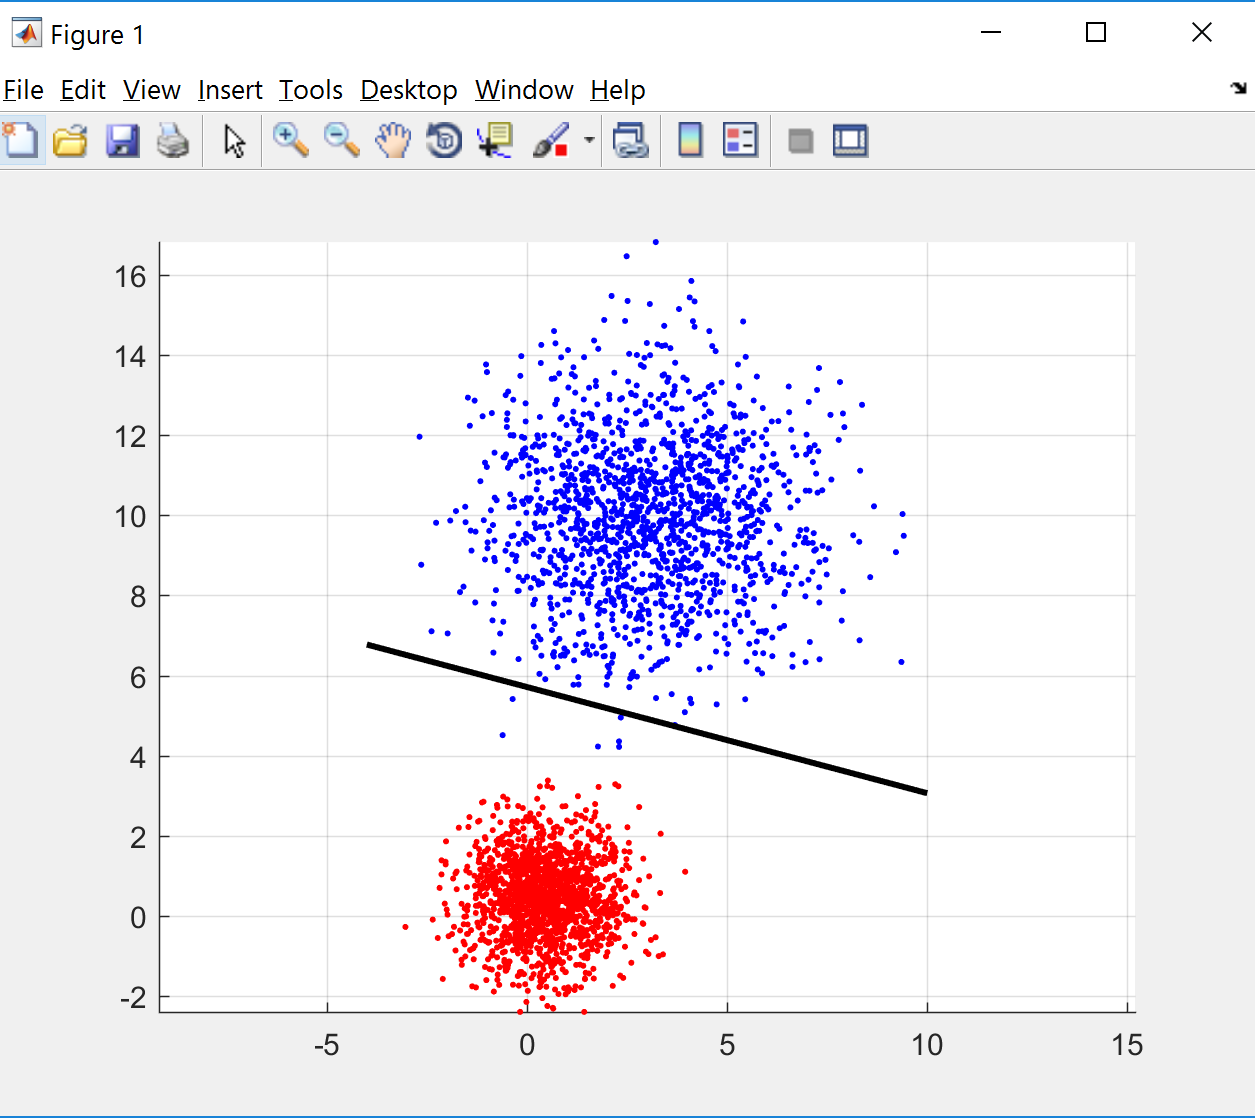
\includegraphics[width=100mm,scale=0.3]{ridge}\\
\end{figure}

\begin{figure}
\caption{SVM C = 0.01}
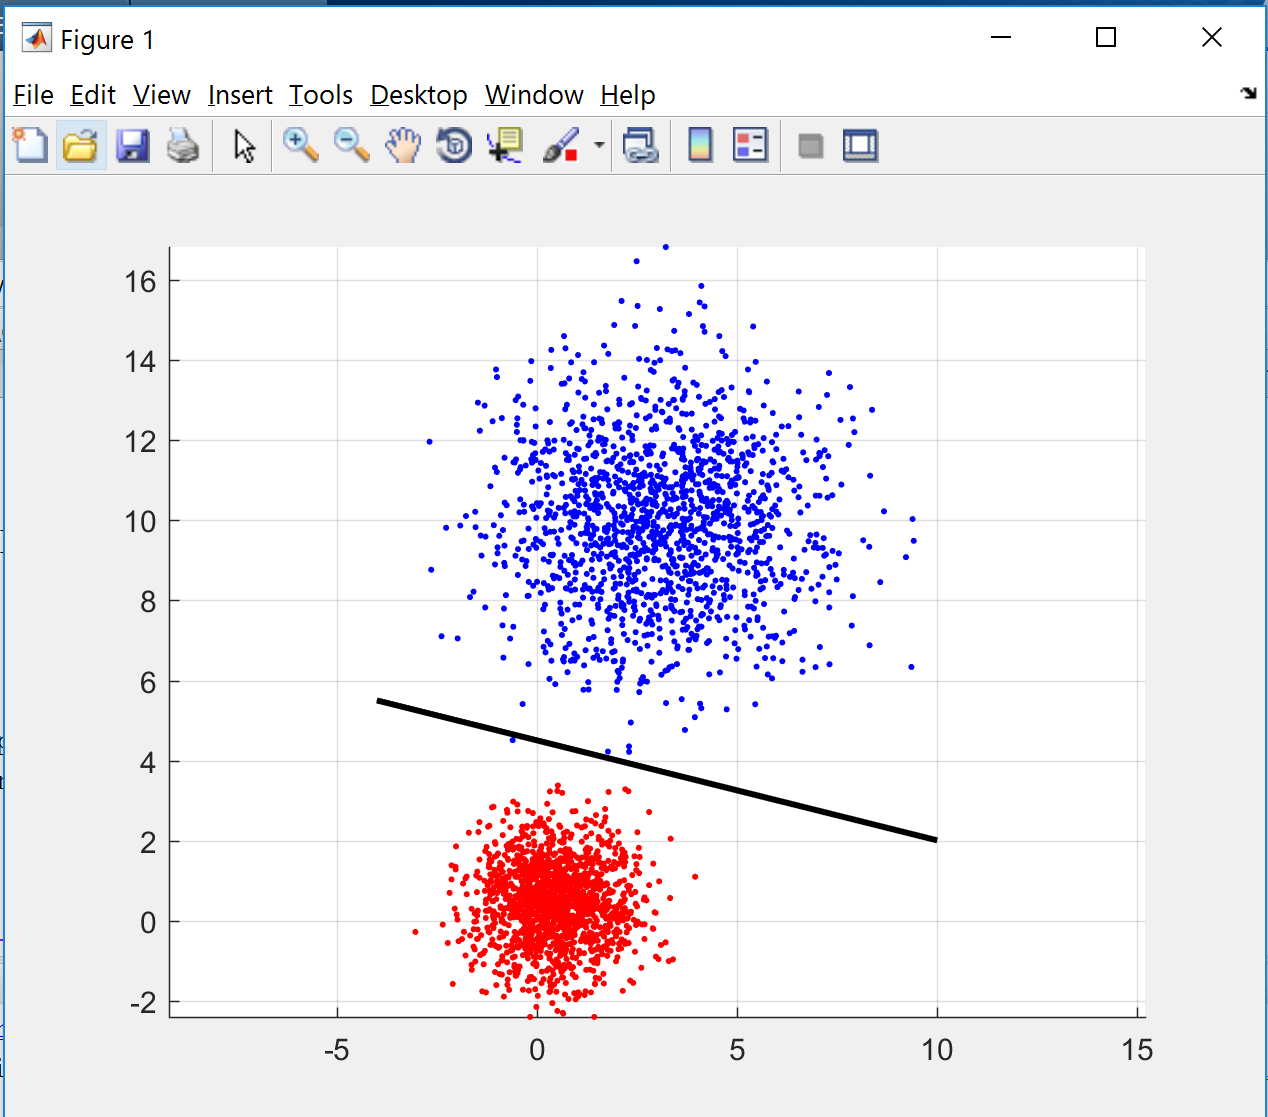
\includegraphics[width=100mm,scale=0.3]{svm001}\\
\end{figure}

\begin{figure}
\caption{SVM C = 100}
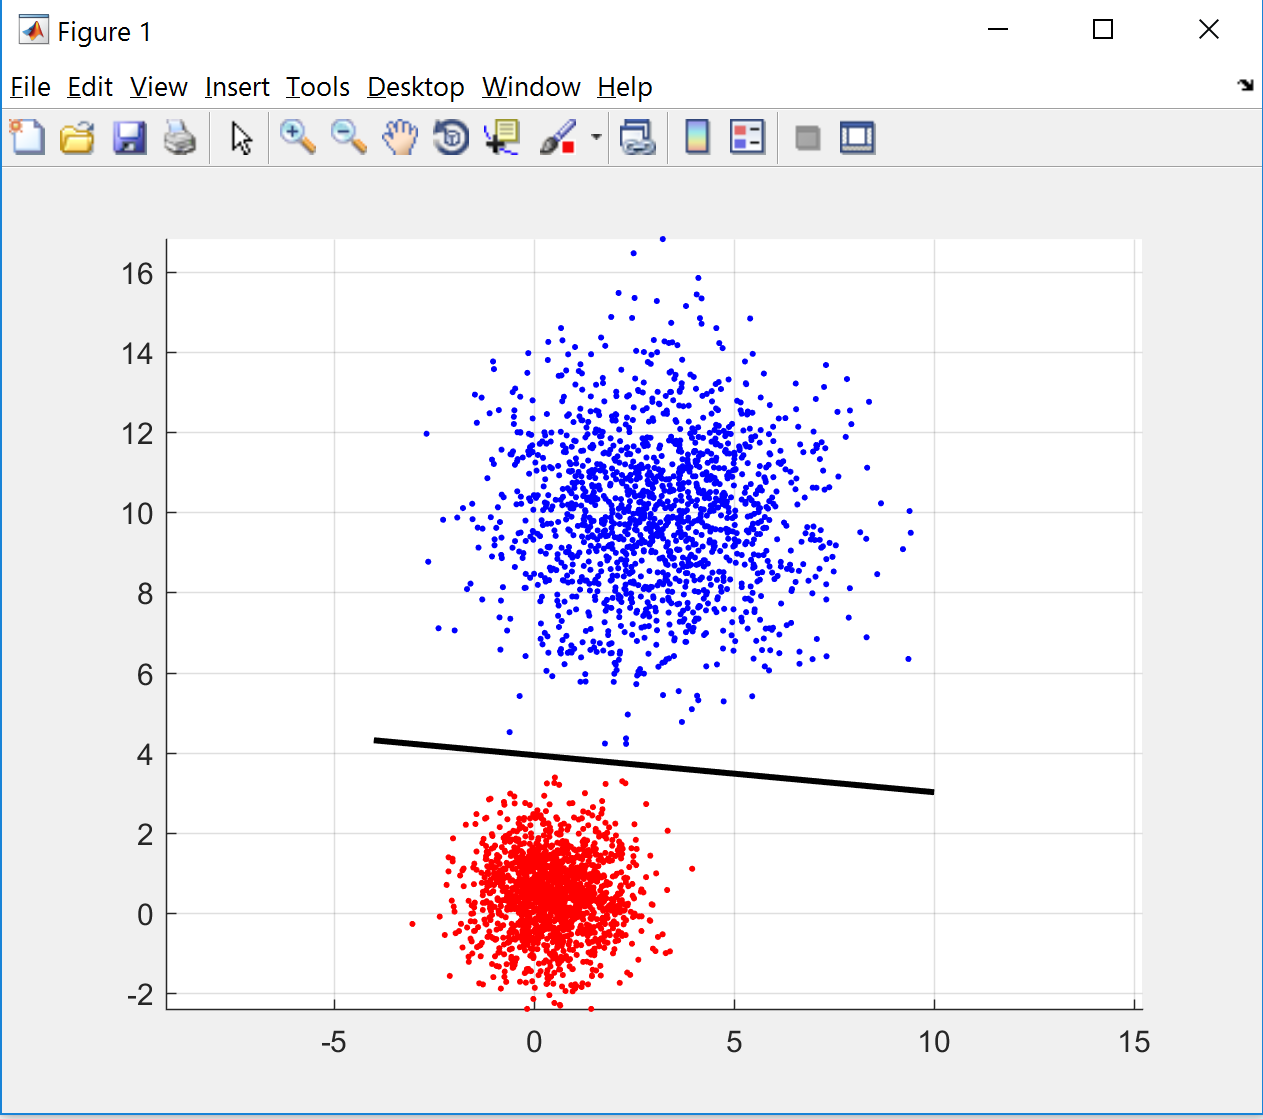
\includegraphics[width=100mm,scale=0.3]{svm100}\\
\end{figure}

\begin{figure}
\caption{Perceptron}
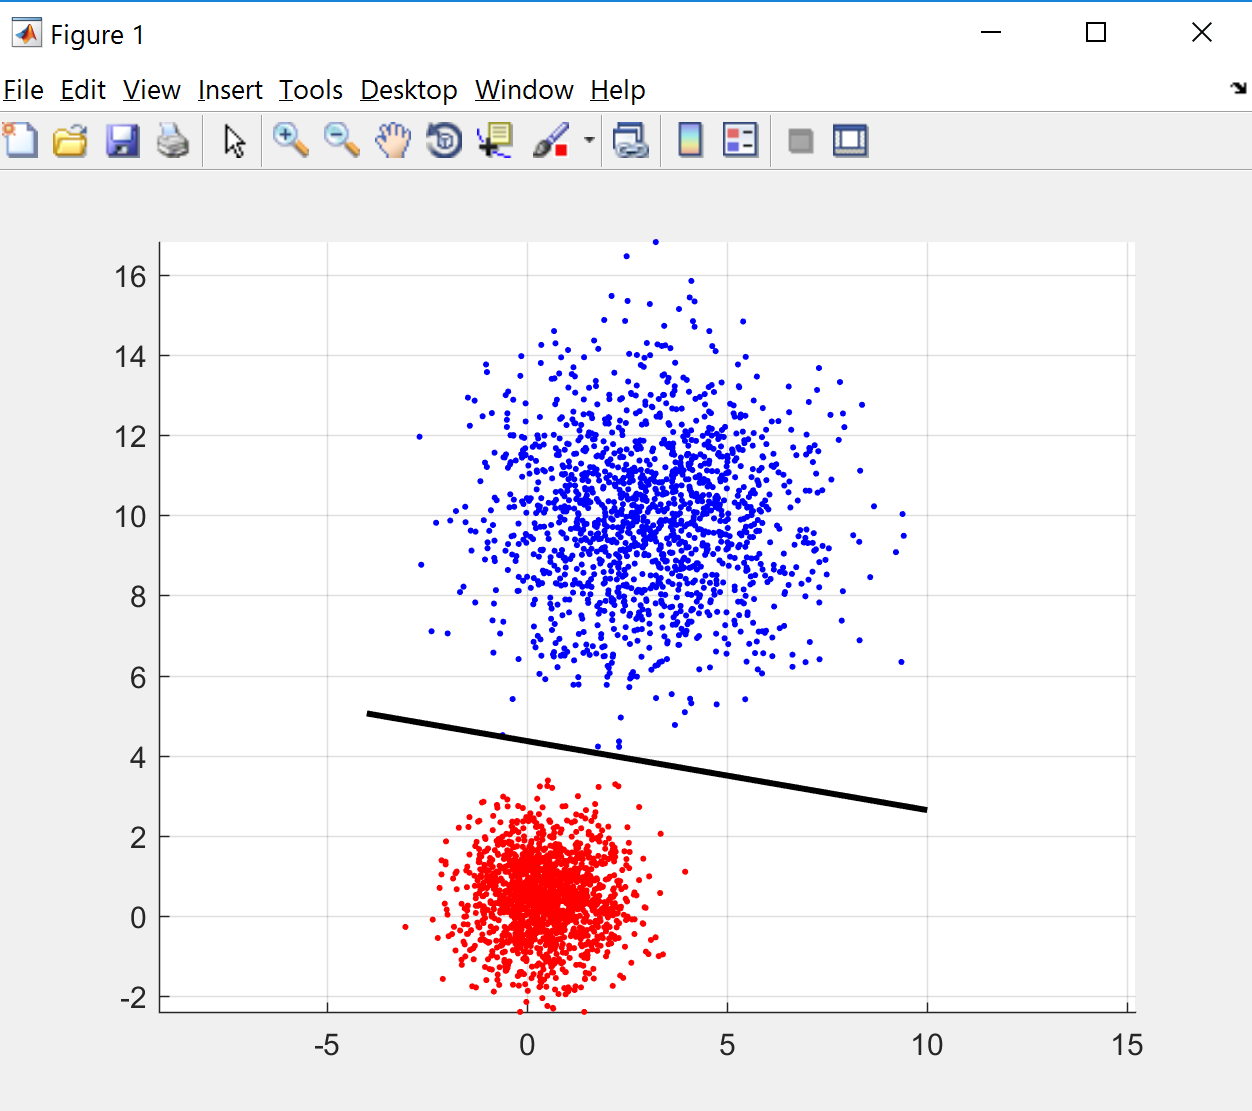
\includegraphics[width=100mm,scale=0.3]{perceptron}\\
\end{figure}

\end{center}



\end{itemize}



\end{document} 